% Options for packages loaded elsewhere
\PassOptionsToPackage{unicode}{hyperref}
\PassOptionsToPackage{hyphens}{url}
%
\documentclass[
]{article}
\usepackage{lmodern}
\usepackage{amssymb,amsmath}
\usepackage{ifxetex,ifluatex}
\ifnum 0\ifxetex 1\fi\ifluatex 1\fi=0 % if pdftex
  \usepackage[T1]{fontenc}
  \usepackage[utf8]{inputenc}
  \usepackage{textcomp} % provide euro and other symbols
\else % if luatex or xetex
  \usepackage{unicode-math}
  \defaultfontfeatures{Scale=MatchLowercase}
  \defaultfontfeatures[\rmfamily]{Ligatures=TeX,Scale=1}
\fi
% Use upquote if available, for straight quotes in verbatim environments
\IfFileExists{upquote.sty}{\usepackage{upquote}}{}
\IfFileExists{microtype.sty}{% use microtype if available
  \usepackage[]{microtype}
  \UseMicrotypeSet[protrusion]{basicmath} % disable protrusion for tt fonts
}{}
\makeatletter
\@ifundefined{KOMAClassName}{% if non-KOMA class
  \IfFileExists{parskip.sty}{%
    \usepackage{parskip}
  }{% else
    \setlength{\parindent}{0pt}
    \setlength{\parskip}{6pt plus 2pt minus 1pt}}
}{% if KOMA class
  \KOMAoptions{parskip=half}}
\makeatother
\usepackage{xcolor}
\IfFileExists{xurl.sty}{\usepackage{xurl}}{} % add URL line breaks if available
\IfFileExists{bookmark.sty}{\usepackage{bookmark}}{\usepackage{hyperref}}
\hypersetup{
  pdftitle={Sars vs.~COVID-19},
  pdfauthor={Melodie Irvin, mki77},
  hidelinks,
  pdfcreator={LaTeX via pandoc}}
\urlstyle{same} % disable monospaced font for URLs
\usepackage[margin=1in]{geometry}
\usepackage{color}
\usepackage{fancyvrb}
\newcommand{\VerbBar}{|}
\newcommand{\VERB}{\Verb[commandchars=\\\{\}]}
\DefineVerbatimEnvironment{Highlighting}{Verbatim}{commandchars=\\\{\}}
% Add ',fontsize=\small' for more characters per line
\usepackage{framed}
\definecolor{shadecolor}{RGB}{248,248,248}
\newenvironment{Shaded}{\begin{snugshade}}{\end{snugshade}}
\newcommand{\AlertTok}[1]{\textcolor[rgb]{0.94,0.16,0.16}{#1}}
\newcommand{\AnnotationTok}[1]{\textcolor[rgb]{0.56,0.35,0.01}{\textbf{\textit{#1}}}}
\newcommand{\AttributeTok}[1]{\textcolor[rgb]{0.77,0.63,0.00}{#1}}
\newcommand{\BaseNTok}[1]{\textcolor[rgb]{0.00,0.00,0.81}{#1}}
\newcommand{\BuiltInTok}[1]{#1}
\newcommand{\CharTok}[1]{\textcolor[rgb]{0.31,0.60,0.02}{#1}}
\newcommand{\CommentTok}[1]{\textcolor[rgb]{0.56,0.35,0.01}{\textit{#1}}}
\newcommand{\CommentVarTok}[1]{\textcolor[rgb]{0.56,0.35,0.01}{\textbf{\textit{#1}}}}
\newcommand{\ConstantTok}[1]{\textcolor[rgb]{0.00,0.00,0.00}{#1}}
\newcommand{\ControlFlowTok}[1]{\textcolor[rgb]{0.13,0.29,0.53}{\textbf{#1}}}
\newcommand{\DataTypeTok}[1]{\textcolor[rgb]{0.13,0.29,0.53}{#1}}
\newcommand{\DecValTok}[1]{\textcolor[rgb]{0.00,0.00,0.81}{#1}}
\newcommand{\DocumentationTok}[1]{\textcolor[rgb]{0.56,0.35,0.01}{\textbf{\textit{#1}}}}
\newcommand{\ErrorTok}[1]{\textcolor[rgb]{0.64,0.00,0.00}{\textbf{#1}}}
\newcommand{\ExtensionTok}[1]{#1}
\newcommand{\FloatTok}[1]{\textcolor[rgb]{0.00,0.00,0.81}{#1}}
\newcommand{\FunctionTok}[1]{\textcolor[rgb]{0.00,0.00,0.00}{#1}}
\newcommand{\ImportTok}[1]{#1}
\newcommand{\InformationTok}[1]{\textcolor[rgb]{0.56,0.35,0.01}{\textbf{\textit{#1}}}}
\newcommand{\KeywordTok}[1]{\textcolor[rgb]{0.13,0.29,0.53}{\textbf{#1}}}
\newcommand{\NormalTok}[1]{#1}
\newcommand{\OperatorTok}[1]{\textcolor[rgb]{0.81,0.36,0.00}{\textbf{#1}}}
\newcommand{\OtherTok}[1]{\textcolor[rgb]{0.56,0.35,0.01}{#1}}
\newcommand{\PreprocessorTok}[1]{\textcolor[rgb]{0.56,0.35,0.01}{\textit{#1}}}
\newcommand{\RegionMarkerTok}[1]{#1}
\newcommand{\SpecialCharTok}[1]{\textcolor[rgb]{0.00,0.00,0.00}{#1}}
\newcommand{\SpecialStringTok}[1]{\textcolor[rgb]{0.31,0.60,0.02}{#1}}
\newcommand{\StringTok}[1]{\textcolor[rgb]{0.31,0.60,0.02}{#1}}
\newcommand{\VariableTok}[1]{\textcolor[rgb]{0.00,0.00,0.00}{#1}}
\newcommand{\VerbatimStringTok}[1]{\textcolor[rgb]{0.31,0.60,0.02}{#1}}
\newcommand{\WarningTok}[1]{\textcolor[rgb]{0.56,0.35,0.01}{\textbf{\textit{#1}}}}
\usepackage{graphicx,grffile}
\makeatletter
\def\maxwidth{\ifdim\Gin@nat@width>\linewidth\linewidth\else\Gin@nat@width\fi}
\def\maxheight{\ifdim\Gin@nat@height>\textheight\textheight\else\Gin@nat@height\fi}
\makeatother
% Scale images if necessary, so that they will not overflow the page
% margins by default, and it is still possible to overwrite the defaults
% using explicit options in \includegraphics[width, height, ...]{}
\setkeys{Gin}{width=\maxwidth,height=\maxheight,keepaspectratio}
% Set default figure placement to htbp
\makeatletter
\def\fps@figure{htbp}
\makeatother
\setlength{\emergencystretch}{3em} % prevent overfull lines
\providecommand{\tightlist}{%
  \setlength{\itemsep}{0pt}\setlength{\parskip}{0pt}}
\setcounter{secnumdepth}{-\maxdimen} % remove section numbering
\usepackage{booktabs}
\usepackage{longtable}
\usepackage{array}
\usepackage{multirow}
\usepackage{wrapfig}
\usepackage{float}
\usepackage{colortbl}
\usepackage{pdflscape}
\usepackage{tabu}
\usepackage{threeparttable}
\usepackage{threeparttablex}
\usepackage[normalem]{ulem}
\usepackage{makecell}
\usepackage{xcolor}

\title{Sars vs.~COVID-19}
\author{Melodie Irvin, mki77}
\date{}

\begin{document}
\maketitle

Virology has always excited me, and with the coronavirus looming around
everywhere we go, I found it compelling to compare the current data
regarding the deaths and confirmed cases of COVID-19 with it's sister
virus, SARS-CoV from 2003. Considering they are of the same genus and
species of virus, I was expecting to find similar results regarding the
number of deaths and rate of infection. As you will see, that is not at
all the case. The Sars dataset was gathered from Kaggle while the COVID
dataset was taken from ourworldindata.org. Both were combined in Excel
prior to importing. The COVID dataset is up-to-date as of March 13,
2020.

\begin{Shaded}
\begin{Highlighting}[]
\KeywordTok{options}\NormalTok{(}\DataTypeTok{repos=}\StringTok{"https://cran.rstudio.com"}\NormalTok{ )}
\KeywordTok{library}\NormalTok{(dplyr)}
\KeywordTok{library}\NormalTok{(ggplot2)}
\KeywordTok{library}\NormalTok{(readxl)}
\NormalTok{COVID_and_SARS <-}\StringTok{ }\KeywordTok{read_excel}\NormalTok{(}\StringTok{"C:/Users/Melodie/Desktop/COVID_and_SARS.xlsx"}\NormalTok{)}
\NormalTok{COVID_and_SARS<-COVID_and_SARS}\OperatorTok\KeywordTok{slice}\NormalTok{(}\DecValTok{1}\OperatorTok{:}\DecValTok{70}\NormalTok{)}
\NormalTok{COVID <-COVID_and_SARS}\OperatorTok\KeywordTok{select}\NormalTok{(Date.Rank, Sum.of.COVID.Confirmed, Sum.of.COVID.Deaths)}
\NormalTok{SARS<-COVID_and_SARS}\OperatorTok\KeywordTok{select}\NormalTok{(}\DataTypeTok{by=}\OperatorTok{-}\KeywordTok{c}\NormalTok{(Sum.of.COVID.Confirmed, Sum.of.COVID.Deaths))}\OperatorTok
\StringTok{  }\KeywordTok{select}\NormalTok{(}\DataTypeTok{Day=}\NormalTok{Date.Rank, Sum.of.Sars.Deaths, Sum.of.Sars.Confirmed)}
\end{Highlighting}
\end{Shaded}

\begin{Shaded}
\begin{Highlighting}[]
\NormalTok{FULL<-}\StringTok{ }\KeywordTok{full_join}\NormalTok{(COVID, SARS, }\DataTypeTok{by=}\KeywordTok{c}\NormalTok{(}\StringTok{"Date.Rank"}\NormalTok{=}\StringTok{"Day"}\NormalTok{))}
\NormalTok{FULL_}\DecValTok{2}\NormalTok{ <-FULL}\OperatorTok\KeywordTok{mutate}\NormalTok{(}
  \DataTypeTok{Week.Number=} \KeywordTok{case_when}\NormalTok{(}
    \KeywordTok{between}\NormalTok{(}\StringTok{`}\DataTypeTok{Date.Rank}\StringTok{`}\NormalTok{,}\DecValTok{1}\NormalTok{,}\DecValTok{7}\NormalTok{)}\OperatorTok{~}\StringTok{"Week One"}\NormalTok{,}
    \KeywordTok{between}\NormalTok{(}\StringTok{`}\DataTypeTok{Date.Rank}\StringTok{`}\NormalTok{,}\DecValTok{8}\NormalTok{,}\DecValTok{14}\NormalTok{)}\OperatorTok{~}\StringTok{"Week Two"}\NormalTok{,}
    \KeywordTok{between}\NormalTok{(}\StringTok{`}\DataTypeTok{Date.Rank}\StringTok{`}\NormalTok{,}\DecValTok{15}\NormalTok{,}\DecValTok{21}\NormalTok{)}\OperatorTok{~}\StringTok{"Week Three"}\NormalTok{,}
    \KeywordTok{between}\NormalTok{(}\StringTok{`}\DataTypeTok{Date.Rank}\StringTok{`}\NormalTok{,}\DecValTok{22}\NormalTok{,}\DecValTok{28}\NormalTok{)}\OperatorTok{~}\StringTok{"Week Four"}\NormalTok{,}
    \KeywordTok{between}\NormalTok{(}\StringTok{`}\DataTypeTok{Date.Rank}\StringTok{`}\NormalTok{,}\DecValTok{29}\NormalTok{,}\DecValTok{35}\NormalTok{)}\OperatorTok{~}\StringTok{"Week Five"}\NormalTok{,}
    \KeywordTok{between}\NormalTok{(}\StringTok{`}\DataTypeTok{Date.Rank}\StringTok{`}\NormalTok{,}\DecValTok{36}\NormalTok{,}\DecValTok{42}\NormalTok{)}\OperatorTok{~}\StringTok{"Week Six"}\NormalTok{,}
    \KeywordTok{between}\NormalTok{(}\StringTok{`}\DataTypeTok{Date.Rank}\StringTok{`}\NormalTok{,}\DecValTok{43}\NormalTok{,}\DecValTok{49}\NormalTok{)}\OperatorTok{~}\StringTok{"Week Seven"}\NormalTok{,}
    \KeywordTok{between}\NormalTok{(}\StringTok{`}\DataTypeTok{Date.Rank}\StringTok{`}\NormalTok{,}\DecValTok{50}\NormalTok{,}\DecValTok{56}\NormalTok{)}\OperatorTok{~}\StringTok{"Week Eight"}\NormalTok{,}
    \KeywordTok{between}\NormalTok{(}\StringTok{`}\DataTypeTok{Date.Rank}\StringTok{`}\NormalTok{,}\DecValTok{57}\NormalTok{,}\DecValTok{63}\NormalTok{)}\OperatorTok{~}\StringTok{"Week Nine"}\NormalTok{,}
    \KeywordTok{between}\NormalTok{(}\StringTok{`}\DataTypeTok{Date.Rank}\StringTok{`}\NormalTok{,}\DecValTok{64}\NormalTok{,}\DecValTok{70}\NormalTok{)}\OperatorTok{~}\StringTok{"Week Ten"}\NormalTok{,}
    \KeywordTok{between}\NormalTok{(}\StringTok{`}\DataTypeTok{Date.Rank}\StringTok{`}\NormalTok{,}\DecValTok{71}\NormalTok{,}\DecValTok{77}\NormalTok{)}\OperatorTok{~}\StringTok{"Week Eleven"}\NormalTok{,}
    \KeywordTok{between}\NormalTok{(}\StringTok{`}\DataTypeTok{Date.Rank}\StringTok{`}\NormalTok{,}\DecValTok{78}\NormalTok{,}\DecValTok{84}\NormalTok{)}\OperatorTok{~}\StringTok{"Week Twelve"}\NormalTok{,}
    \KeywordTok{between}\NormalTok{(}\StringTok{`}\DataTypeTok{Date.Rank}\StringTok{`}\NormalTok{,}\DecValTok{85}\NormalTok{,}\DecValTok{91}\NormalTok{)}\OperatorTok{~}\StringTok{"Week Thirteen"}\NormalTok{,}
    \KeywordTok{between}\NormalTok{(}\StringTok{`}\DataTypeTok{Date.Rank}\StringTok{`}\NormalTok{,}\DecValTok{92}\NormalTok{,}\DecValTok{96}\NormalTok{)}\OperatorTok{~}\StringTok{"Week Fourteen"}
\NormalTok{  )}
\NormalTok{)}\OperatorTok
\StringTok{  }\KeywordTok{select}\NormalTok{(Date.Rank, Sum.of.COVID.Confirmed, Sum.of.Sars.Confirmed, Sum.of.COVID.Deaths,   Sum.of.Sars.Deaths, Week.Number)}
\NormalTok{FULL_New<-FULL_}\DecValTok{2}\OperatorTok\KeywordTok{arrange}\NormalTok{(Date.Rank)}\OperatorTok
\StringTok{  }\KeywordTok{mutate}\NormalTok{(}\DataTypeTok{COVID.New.Cases=}\NormalTok{Sum.of.COVID.Confirmed}\OperatorTok{-}\KeywordTok{lag}\NormalTok{(Sum.of.COVID.Confirmed))}\OperatorTok
\StringTok{  }\KeywordTok{mutate}\NormalTok{(}\DataTypeTok{COVID.New.Deaths=}\NormalTok{Sum.of.COVID.Deaths}\OperatorTok{-}\KeywordTok{lag}\NormalTok{(Sum.of.COVID.Deaths))}\OperatorTok
\StringTok{  }\KeywordTok{mutate}\NormalTok{(}\DataTypeTok{Sars.New.Cases=}\NormalTok{Sum.of.Sars.Confirmed}\OperatorTok{-}\KeywordTok{lag}\NormalTok{(Sum.of.Sars.Confirmed))}\OperatorTok
\StringTok{  }\KeywordTok{mutate}\NormalTok{(}\DataTypeTok{Sars.New.Deaths=}\NormalTok{ Sum.of.Sars.Deaths}\OperatorTok{-}\KeywordTok{lag}\NormalTok{(Sum.of.Sars.Deaths))}\OperatorTok
\StringTok{  }\KeywordTok{select}\NormalTok{(Date.Rank,Sum.of.COVID.Confirmed, Sum.of.Sars.Confirmed, Sum.of.COVID.Deaths, Sum.of.Sars.Deaths,}
\NormalTok{         COVID.New.Cases, Sars.New.Cases, COVID.New.Deaths, Sars.New.Deaths, Week.Number)}
\end{Highlighting}
\end{Shaded}

Given that this data is tidy, the pivot\_longer and pivot\_wider
fuctions will be used in another section. The object of using those
functions, however, is to organize data so that each observation has
it's own row and each variable has it's own column. I chose to do a
full\_join of the data because I imported a single dataset and wanted to
ensure I kept all components, therefore, no results were lost. A few
additional columns were made for gathering summary statistics as well as
to create a categorical variable.

\begin{Shaded}
\begin{Highlighting}[]
\NormalTok{FULL_New}\OperatorTok\StringTok{ }\KeywordTok{filter}\NormalTok{(}\KeywordTok{between}\NormalTok{(Date.Rank,}\DecValTok{25}\NormalTok{,}\DecValTok{50}\NormalTok{))}
\end{Highlighting}
\end{Shaded}

\begin{verbatim}
## # A tibble: 26 x 10
##    Date.Rank Sum.of.COVID.Co~ Sum.of.Sars.Con~ Sum.of.COVID.De~ Sum.of.Sars.Dea~
##        <dbl>            <dbl>            <dbl>            <dbl>            <dbl>
##  1        25            49053             3233             1383              144
##  2        26            50580             3298             1526              154
##  3        27            51857             3357             1669              159
##  4        28            71429             3448             1775              165
##  5        29            73332             3595             1873              182
##  6        30            75204             4090             2009              182
##  7        31            75748             4180             2129              217
##  8        32            76769             4561             2247              229
##  9        33            77794             4713             2359              251
## 10        34            78811             4921             2463              263
## # ... with 16 more rows, and 5 more variables: COVID.New.Cases <dbl>,
## #   Sars.New.Cases <dbl>, COVID.New.Deaths <dbl>, Sars.New.Deaths <dbl>,
## #   Week.Number <chr>
\end{verbatim}

\begin{Shaded}
\begin{Highlighting}[]
\NormalTok{FULL_New}\OperatorTok\StringTok{ }\KeywordTok{select}\NormalTok{(Sum.of.COVID.Confirmed,Sum.of.Sars.Confirmed, }\KeywordTok{everything}\NormalTok{())}\OperatorTok
\StringTok{  }\KeywordTok{arrange}\NormalTok{(}\KeywordTok{desc}\NormalTok{(Sum.of.COVID.Confirmed))}
\end{Highlighting}
\end{Shaded}

\begin{verbatim}
## # A tibble: 70 x 10
##    Sum.of.COVID.Co~ Sum.of.Sars.Con~ Date.Rank Sum.of.COVID.De~ Sum.of.Sars.Dea~
##               <dbl>            <dbl>     <dbl>            <dbl>            <dbl>
##  1           132758             7624        53             4955              610
##  2           125260             7569        52             4613              597
##  3           118319             7467        51             4292              586
##  4           113702             7445        50             4012              572
##  5           109577             7404        49             3809              551
##  6           105592             7280        48             3584              525
##  7           101927             7178        47             3486              513
##  8            98192             7074        46             3380              505
##  9            95324             6923        45             3280              494
## 10            93090             6800        44             3198              477
## # ... with 60 more rows, and 5 more variables: COVID.New.Cases <dbl>,
## #   Sars.New.Cases <dbl>, COVID.New.Deaths <dbl>, Sars.New.Deaths <dbl>,
## #   Week.Number <chr>
\end{verbatim}

\begin{Shaded}
\begin{Highlighting}[]
\NormalTok{FULL_New}\OperatorTok
\StringTok{  }\KeywordTok{slice}\NormalTok{(}\DecValTok{1}\OperatorTok{:}\DecValTok{53}\NormalTok{)}\OperatorTok\KeywordTok{group_by}\NormalTok{(Week.Number)}\OperatorTok
\StringTok{  }\KeywordTok{summarize}\NormalTok{(}\DataTypeTok{mean_COVNew=}\KeywordTok{mean}\NormalTok{(COVID.New.Cases,}\DataTypeTok{na.rm=}\NormalTok{T), }\DataTypeTok{sd_COVNew=}\KeywordTok{sd}\NormalTok{(COVID.New.Cases, }\DataTypeTok{na.rm=}\NormalTok{T))}
\end{Highlighting}
\end{Shaded}

\begin{verbatim}
## # A tibble: 8 x 3
##   Week.Number mean_COVNew sd_COVNew
##   <chr>             <dbl>     <dbl>
## 1 Week Eight        5795.     1672.
## 2 Week Five         1129.      563.
## 3 Week Four         4411.     6698.
## 4 Week One           419.      286.
## 5 Week Seven        2947       847.
## 6 Week Six          1374.      402.
## 7 Week Three        3309       423.
## 8 Week Two          2085.      484.
\end{verbatim}

\begin{Shaded}
\begin{Highlighting}[]
\NormalTok{FULL_New}\OperatorTok
\StringTok{  }\KeywordTok{slice}\NormalTok{(}\DecValTok{1}\OperatorTok{:}\DecValTok{53}\NormalTok{)}\OperatorTok\KeywordTok{summarize}\NormalTok{(}\KeywordTok{median}\NormalTok{(Sum.of.COVID.Confirmed))}
\end{Highlighting}
\end{Shaded}

\begin{verbatim}
## # A tibble: 1 x 1
##   `median(Sum.of.COVID.Confirmed)`
##                              <dbl>
## 1                            51857
\end{verbatim}

\begin{Shaded}
\begin{Highlighting}[]
\NormalTok{FULL_New}\OperatorTok
\StringTok{  }\KeywordTok{summarize}\NormalTok{(}\KeywordTok{median}\NormalTok{(Sum.of.Sars.Confirmed))}
\end{Highlighting}
\end{Shaded}

\begin{verbatim}
## # A tibble: 1 x 1
##   `median(Sum.of.Sars.Confirmed)`
##                             <dbl>
## 1                           5212.
\end{verbatim}

\begin{Shaded}
\begin{Highlighting}[]
\NormalTok{FULL_New}\OperatorTok
\StringTok{  }\KeywordTok{slice}\NormalTok{(}\DecValTok{1}\OperatorTok{:}\DecValTok{53}\NormalTok{)}\OperatorTok\KeywordTok{summarize}\NormalTok{(}\KeywordTok{first}\NormalTok{(Sum.of.COVID.Deaths), }\KeywordTok{last}\NormalTok{(Sum.of.COVID.Deaths), }\DataTypeTok{n_Week=}\KeywordTok{n_distinct}\NormalTok{(Week.Number))}
\end{Highlighting}
\end{Shaded}

\begin{verbatim}
## # A tibble: 1 x 3
##   `first(Sum.of.COVID.Deaths)` `last(Sum.of.COVID.Deaths)` n_Week
##                          <dbl>                       <dbl>  <int>
## 1                            6                        4955      8
\end{verbatim}

\begin{Shaded}
\begin{Highlighting}[]
\NormalTok{FULL_New}\OperatorTok\KeywordTok{summarize}\NormalTok{(}\KeywordTok{first}\NormalTok{(Sum.of.Sars.Deaths), }\KeywordTok{last}\NormalTok{(Sum.of.Sars.Deaths), }\DataTypeTok{n_Week=}\KeywordTok{n_distinct}\NormalTok{(Week.Number))}
\end{Highlighting}
\end{Shaded}

\begin{verbatim}
## # A tibble: 1 x 3
##   `first(Sum.of.Sars.Deaths)` `last(Sum.of.Sars.Deaths)` n_Week
##                         <dbl>                      <dbl>  <int>
## 1                           4                        774     10
\end{verbatim}

\begin{Shaded}
\begin{Highlighting}[]
\NormalTok{FULL_New}\OperatorTok
\StringTok{  }\KeywordTok{group_by}\NormalTok{(Week.Number)}\OperatorTok
\StringTok{  }\KeywordTok{summarize}\NormalTok{(}\DataTypeTok{mean_SARNew=}\KeywordTok{mean}\NormalTok{(Sars.New.Cases,}\DataTypeTok{na.rm=}\NormalTok{T), }\DataTypeTok{sd_SARNew=}\KeywordTok{sd}\NormalTok{(Sars.New.Cases, }\DataTypeTok{na.rm=}\NormalTok{T))}
\end{Highlighting}
\end{Shaded}

\begin{verbatim}
## # A tibble: 10 x 3
##    Week.Number mean_SARNew sd_SARNew
##    <chr>             <dbl>     <dbl>
##  1 Week Eight        52.9      26.5 
##  2 Week Five        237.      146.  
##  3 Week Four         95.9      53.7 
##  4 Week Nine         36.7      17.4 
##  5 Week One          59.2      30.6 
##  6 Week Seven       126.       19.9 
##  7 Week Six         202        65.2 
##  8 Week Ten           9.57      6.53
##  9 Week Three       129.      135.  
## 10 Week Two         193.      288.
\end{verbatim}

\begin{Shaded}
\begin{Highlighting}[]
\NormalTok{FULL_New}\OperatorTok\NormalTok{na.omit}\OperatorTok\KeywordTok{summarize}\NormalTok{(}\KeywordTok{cor}\NormalTok{(Sars.New.Cases, COVID.New.Cases))}
\end{Highlighting}
\end{Shaded}

\begin{verbatim}
## # A tibble: 1 x 1
##   `cor(Sars.New.Cases, COVID.New.Cases)`
##                                    <dbl>
## 1                                 -0.124
\end{verbatim}

\begin{Shaded}
\begin{Highlighting}[]
\NormalTok{FULL_New}\OperatorTok
\StringTok{  }\KeywordTok{slice}\NormalTok{(}\DecValTok{1}\OperatorTok{:}\DecValTok{53}\NormalTok{)}\OperatorTok\KeywordTok{summarize}\NormalTok{(}\DataTypeTok{mean_CNC=}\KeywordTok{mean}\NormalTok{(COVID.New.Cases, }\DataTypeTok{na.rm=}\NormalTok{T), }\KeywordTok{sd}\NormalTok{(COVID.New.Cases, }\DataTypeTok{na.rm=}\NormalTok{T))}
\end{Highlighting}
\end{Shaded}

\begin{verbatim}
## # A tibble: 1 x 2
##   mean_CNC `sd(COVID.New.Cases, na.rm = T)`
##      <dbl>                            <dbl>
## 1    2548.                            2841.
\end{verbatim}

\begin{Shaded}
\begin{Highlighting}[]
\NormalTok{FULL_New}\OperatorTok\NormalTok{na.omit}\OperatorTok\KeywordTok{summarize}\NormalTok{(}\KeywordTok{var}\NormalTok{(COVID.New.Cases, COVID.New.Deaths))}
\end{Highlighting}
\end{Shaded}

\begin{verbatim}
## # A tibble: 1 x 1
##   `var(COVID.New.Cases, COVID.New.Deaths)`
##                                      <dbl>
## 1                                   81616.
\end{verbatim}

Given the amount of numeric varibles in the dataset, I only performed
summary statistics on a few using the core dplyr functions. In order to
find the difference in statistics on a set day, I filtered by date rank
and found that the number of confirmed COVID cases on day 25 was more
than 1500 percent of Sars cases on the same day in 2003. In addition, I
selected the sums of COVID deaths and Sars deaths and arranged it in
descending order of COVID deaths. Considering the COVID dataset was
up-to-date as of March 13 (Day 53), I wanted to compare the values of
both viruses. As of this time, the COVID death rate is around 3.73\%,
while the Sars virus from onset to conclusion resulted in around a
9.56\% death rate. In other words, Sars was not as successful at
spreading to as many hosts as COVID, but the people that contracted Sars
had a higher chance of mortality than ones that have contracted COVID.
The group\_by function allowed me to group the categories based on week
number and further summarize to find the mean and standard deviation of
the variable regarding new cases of COVID per week. As shown, the
highest average new cases for COVID occurred in the most recent week
(week 8), while the highest for Sars came in week four. Considering some
of the variable observations were accumulations, I took the median
number for both regarding the sum of confirmed cases. COVID's median was
51,857 in 53 observations, while Sars median was 5,211 in 70
observations. This can be used as an indicator of the quantity of cases
at half the time; days were used as the factor in this case. First and
last sums of deaths were found to be four on day one and 774 on the last
day for Sars virus. A correlation was done between new cases of Sars and
new cases of COVID and was found to have a slighty negative correlation.

\begin{Shaded}
\begin{Highlighting}[]
\KeywordTok{library}\NormalTok{(tidyverse)}
\KeywordTok{library}\NormalTok{(kableExtra)}
\NormalTok{COOR<-FULL_New}\OperatorTok\NormalTok{na.omit}\OperatorTok\KeywordTok{select_if}\NormalTok{(is.numeric)}
\KeywordTok{kable}\NormalTok{(COOR) }\OperatorTok
\StringTok{  }\KeywordTok{kable_styling}\NormalTok{(}\DataTypeTok{fixed_thead =}\NormalTok{ T)}
\end{Highlighting}
\end{Shaded}

\begin{table}[H]
\centering
\begin{tabular}{r|r|r|r|r|r|r|r|r}
\hline
Date.Rank & Sum.of.COVID.Confirmed & Sum.of.Sars.Confirmed & Sum.of.COVID.Deaths & Sum.of.Sars.Deaths & COVID.New.Cases & Sars.New.Cases & COVID.New.Deaths & Sars.New.Deaths\\
\hline
2 & 314 & 231 & 6 & 4 & 32 & 64 & 0 & 0\\
\hline
3 & 581 & 278 & 17 & 9 & 267 & 47 & 11 & 5\\
\hline
4 & 846 & 317 & 25 & 10 & 265 & 39 & 8 & 1\\
\hline
5 & 1320 & 362 & 41 & 10 & 474 & 45 & 16 & 0\\
\hline
6 & 2014 & 403 & 56 & 11 & 694 & 41 & 15 & 1\\
\hline
7 & 2798 & 522 & 80 & 17 & 784 & 119 & 24 & 6\\
\hline
8 & 4593 & 554 & 106 & 17 & 1795 & 32 & 26 & 0\\
\hline
9 & 6065 & 1392 & 132 & 49 & 1472 & 838 & 26 & 32\\
\hline
10 & 7818 & 1478 & 170 & 53 & 1753 & 86 & 38 & 4\\
\hline
11 & 9826 & 1555 & 213 & 53 & 2008 & 77 & 43 & 0\\
\hline
12 & 11953 & 1619 & 259 & 54 & 2127 & 64 & 46 & 1\\
\hline
13 & 14557 & 1690 & 305 & 58 & 2604 & 71 & 46 & 4\\
\hline
14 & 17391 & 1871 & 362 & 62 & 2834 & 181 & 57 & 4\\
\hline
15 & 20630 & 2289 & 426 & 78 & 3239 & 418 & 64 & 16\\
\hline
16 & 24544 & 2338 & 492 & 79 & 3914 & 49 & 66 & 1\\
\hline
17 & 28276 & 2419 & 565 & 84 & 3732 & 81 & 73 & 5\\
\hline
18 & 31481 & 2479 & 638 & 89 & 3205 & 60 & 73 & 5\\
\hline
19 & 34886 & 2660 & 724 & 98 & 3405 & 181 & 86 & 9\\
\hline
20 & 37558 & 2725 & 813 & 103 & 2672 & 65 & 89 & 5\\
\hline
21 & 40554 & 2777 & 910 & 106 & 2996 & 52 & 97 & 3\\
\hline
22 & 43103 & 2843 & 1018 & 111 & 2549 & 66 & 108 & 5\\
\hline
23 & 45171 & 2952 & 1115 & 116 & 2068 & 109 & 97 & 5\\
\hline
24 & 46997 & 3022 & 1369 & 119 & 1826 & 70 & 254 & 3\\
\hline
25 & 49053 & 3233 & 1383 & 144 & 2056 & 211 & 14 & 25\\
\hline
26 & 50580 & 3298 & 1526 & 154 & 1527 & 65 & 143 & 10\\
\hline
27 & 51857 & 3357 & 1669 & 159 & 1277 & 59 & 143 & 5\\
\hline
28 & 71429 & 3448 & 1775 & 165 & 19572 & 91 & 106 & 6\\
\hline
29 & 73332 & 3595 & 1873 & 182 & 1903 & 147 & 98 & 17\\
\hline
30 & 75204 & 4090 & 2009 & 182 & 1872 & 495 & 136 & 0\\
\hline
31 & 75748 & 4180 & 2129 & 217 & 544 & 90 & 120 & 35\\
\hline
32 & 76769 & 4561 & 2247 & 229 & 1021 & 381 & 118 & 12\\
\hline
33 & 77794 & 4713 & 2359 & 251 & 1025 & 152 & 112 & 22\\
\hline
34 & 78811 & 4921 & 2463 & 263 & 1017 & 208 & 104 & 12\\
\hline
35 & 79331 & 5105 & 2618 & 274 & 520 & 184 & 155 & 11\\
\hline
36 & 80239 & 5318 & 2700 & 293 & 908 & 213 & 82 & 19\\
\hline
37 & 81109 & 5504 & 2762 & 321 & 870 & 186 & 62 & 28\\
\hline
38 & 82294 & 5688 & 2804 & 353 & 1185 & 184 & 42 & 32\\
\hline
39 & 83652 & 5870 & 2858 & 372 & 1358 & 182 & 54 & 19\\
\hline
40 & 85403 & 6211 & 2924 & 391 & 1751 & 341 & 66 & 19\\
\hline
41 & 87137 & 6349 & 2977 & 417 & 1734 & 138 & 53 & 26\\
\hline
42 & 88948 & 6519 & 3043 & 435 & 1811 & 170 & 66 & 18\\
\hline
43 & 90869 & 6671 & 3112 & 460 & 1921 & 152 & 69 & 25\\
\hline
44 & 93090 & 6800 & 3198 & 477 & 2221 & 129 & 86 & 17\\
\hline
45 & 95324 & 6923 & 3280 & 494 & 2234 & 123 & 82 & 17\\
\hline
46 & 98192 & 7074 & 3380 & 505 & 2868 & 151 & 100 & 11\\
\hline
47 & 101927 & 7178 & 3486 & 513 & 3735 & 104 & 106 & 8\\
\hline
48 & 105592 & 7280 & 3584 & 525 & 3665 & 102 & 98 & 12\\
\hline
49 & 109577 & 7404 & 3809 & 551 & 3985 & 124 & 225 & 26\\
\hline
50 & 113702 & 7445 & 4012 & 572 & 4125 & 41 & 203 & 21\\
\hline
51 & 118319 & 7467 & 4292 & 586 & 4617 & 22 & 280 & 14\\
\hline
52 & 125260 & 7569 & 4613 & 597 & 6941 & 102 & 321 & 11\\
\hline
53 & 132758 & 7624 & 4955 & 610 & 7498 & 55 & 342 & 13\\
\hline
\end{tabular}
\end{table}

\begin{Shaded}
\begin{Highlighting}[]
\NormalTok{Tidycor<-}\KeywordTok{cor}\NormalTok{(COOR)}\OperatorTok\NormalTok{as.data.frame}\OperatorTok
\StringTok{  }\NormalTok{rownames_to_column}\OperatorTok
\StringTok{  }\KeywordTok{pivot_longer}\NormalTok{(}\OperatorTok{-}\DecValTok{1}\NormalTok{,}\DataTypeTok{names_to=}\StringTok{"name"}\NormalTok{,}\DataTypeTok{values_to=}\StringTok{"correlation"}\NormalTok{)}
\KeywordTok{head}\NormalTok{(Tidycor)}
\end{Highlighting}
\end{Shaded}

\begin{verbatim}
## # A tibble: 6 x 3
##   rowname   name                   correlation
##   <chr>     <chr>                        <dbl>
## 1 Date.Rank Date.Rank                    1    
## 2 Date.Rank Sum.of.COVID.Confirmed       0.991
## 3 Date.Rank Sum.of.Sars.Confirmed        0.995
## 4 Date.Rank Sum.of.COVID.Deaths          0.986
## 5 Date.Rank Sum.of.Sars.Deaths           0.968
## 6 Date.Rank COVID.New.Cases              0.254
\end{verbatim}

\begin{Shaded}
\begin{Highlighting}[]
\NormalTok{Tidycor}\OperatorTok\KeywordTok{ggplot}\NormalTok{(}\KeywordTok{aes}\NormalTok{(rowname,name,}\DataTypeTok{fill=}\NormalTok{correlation))}\OperatorTok{+}
\StringTok{  }\KeywordTok{geom_tile}\NormalTok{()}\OperatorTok{+}
\StringTok{  }\KeywordTok{scale_fill_gradient2}\NormalTok{(}\DataTypeTok{low=}\StringTok{"green"}\NormalTok{,}\DataTypeTok{mid=}\StringTok{"purple"}\NormalTok{,}\DataTypeTok{high=}\StringTok{"blue"}\NormalTok{)}\OperatorTok{+}
\StringTok{  }\KeywordTok{geom_text}\NormalTok{(}\KeywordTok{aes}\NormalTok{(}\DataTypeTok{label=}\KeywordTok{round}\NormalTok{(correlation,}\DecValTok{2}\NormalTok{)),}\DataTypeTok{color =} \StringTok{"black"}\NormalTok{, }\DataTypeTok{size =} \DecValTok{4}\NormalTok{)}\OperatorTok{+}
\StringTok{  }\KeywordTok{theme}\NormalTok{(}\DataTypeTok{axis.text.x =} \KeywordTok{element_text}\NormalTok{(}\DataTypeTok{angle =} \DecValTok{90}\NormalTok{, }\DataTypeTok{hjust =} \DecValTok{1}\NormalTok{))}\OperatorTok{+}\StringTok{ }
\StringTok{  }\KeywordTok{coord_fixed}\NormalTok{()}
\end{Highlighting}
\end{Shaded}

\begin{center}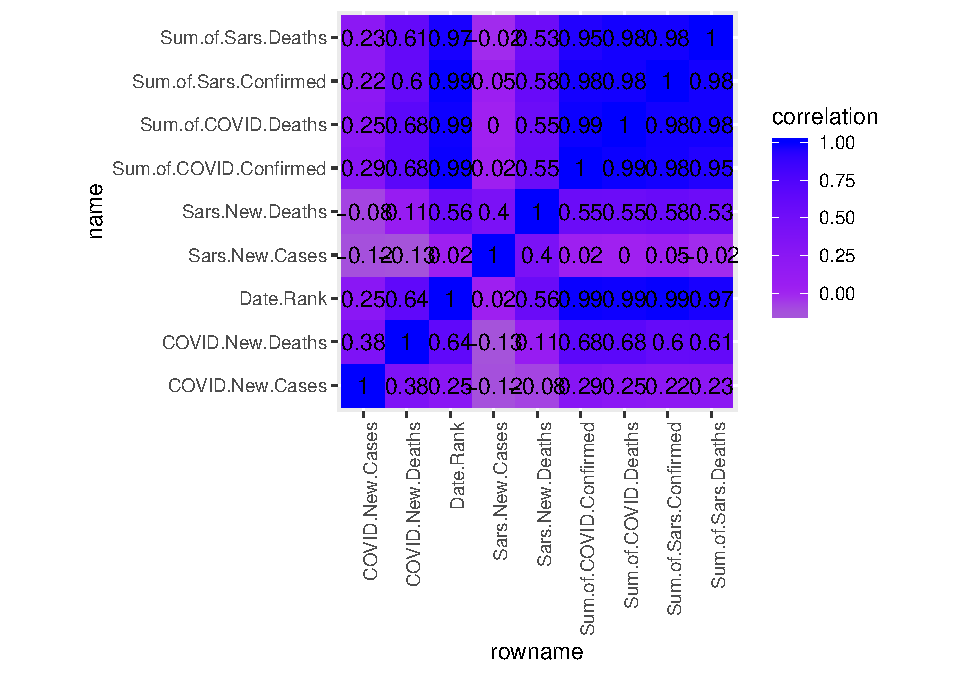
\includegraphics{project1_files/figure-latex/unnamed-chunk-4-1} \end{center}

\begin{Shaded}
\begin{Highlighting}[]
\KeywordTok{ggplot}\NormalTok{(FULL_New, }\KeywordTok{aes}\NormalTok{(Sum.of.Sars.Deaths,Sum.of.Sars.Confirmed, }\DataTypeTok{color=}\NormalTok{Week.Number))}\OperatorTok{+}\KeywordTok{geom_point}\NormalTok{()}\OperatorTok{+}
\StringTok{  }\KeywordTok{theme_light}\NormalTok{()}\OperatorTok{+}
\StringTok{  }\KeywordTok{scale_x_continuous}\NormalTok{(}\DataTypeTok{breaks =}\KeywordTok{seq}\NormalTok{(}\DecValTok{0}\NormalTok{,}\DecValTok{900}\NormalTok{, }\DataTypeTok{by =} \DecValTok{100}\NormalTok{))}\OperatorTok{+}
\StringTok{  }\KeywordTok{scale_y_continuous}\NormalTok{(}\DataTypeTok{lim=}\KeywordTok{c}\NormalTok{(}\DecValTok{0}\NormalTok{,}\DecValTok{9000}\NormalTok{))}\OperatorTok{+}\StringTok{ }
\StringTok{  }\KeywordTok{ggtitle}\NormalTok{(}\StringTok{"Cases and Deaths of Sars-CoV"}\NormalTok{)}
\end{Highlighting}
\end{Shaded}

\begin{center}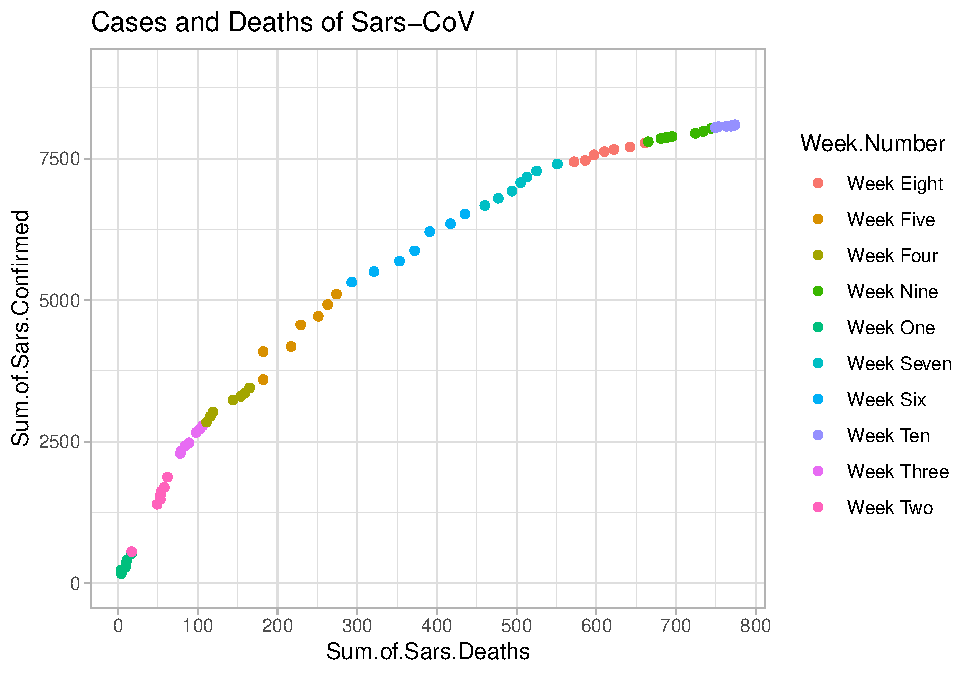
\includegraphics{project1_files/figure-latex/unnamed-chunk-4-2} \end{center}

\begin{Shaded}
\begin{Highlighting}[]
\KeywordTok{ggplot}\NormalTok{(FULL_New, }\KeywordTok{aes}\NormalTok{(}\DataTypeTok{x=}\NormalTok{Sum.of.COVID.Confirmed, }\DataTypeTok{y=}\NormalTok{Sum.of.COVID.Deaths, }\DataTypeTok{fill=}\NormalTok{Week.Number)) }\OperatorTok{+}
\StringTok{  }\KeywordTok{geom_violin}\NormalTok{(}\DataTypeTok{trim=}\NormalTok{F)}\OperatorTok{+}
\StringTok{  }\KeywordTok{geom_boxplot}\NormalTok{(}\DataTypeTok{width=}\NormalTok{.}\DecValTok{1}\NormalTok{)}\OperatorTok{+}
\StringTok{  }\KeywordTok{ggtitle}\NormalTok{(}\StringTok{"Cases and Deaths of COVID-19"}\NormalTok{)}
\end{Highlighting}
\end{Shaded}

\begin{center}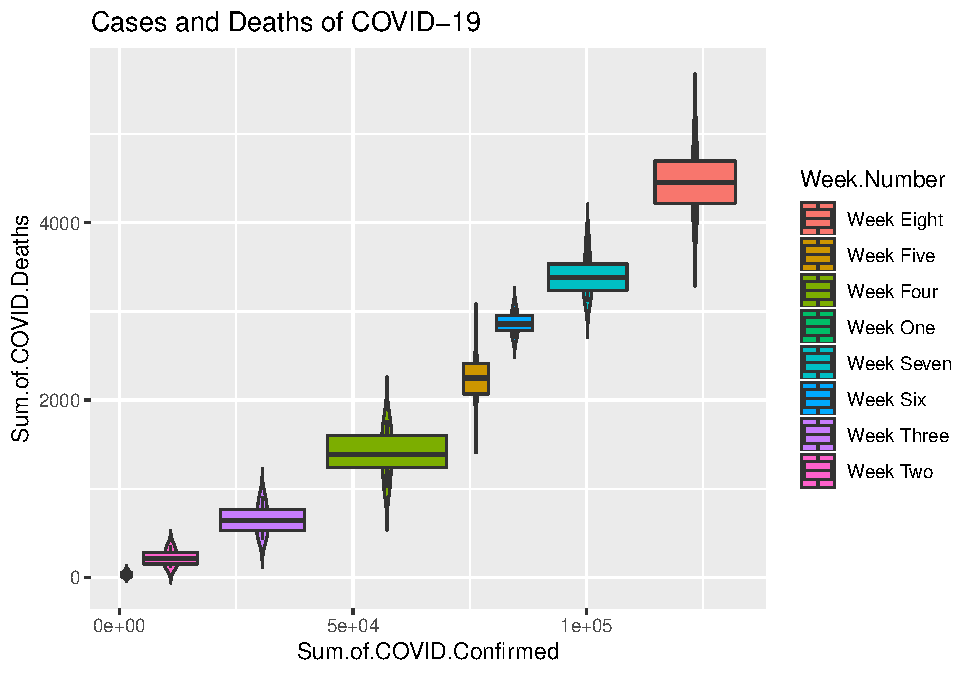
\includegraphics{project1_files/figure-latex/unnamed-chunk-4-3} \end{center}

\begin{Shaded}
\begin{Highlighting}[]
\KeywordTok{ggplot}\NormalTok{(FULL_New, }\KeywordTok{aes}\NormalTok{(}\DataTypeTok{x =}\NormalTok{ Week.Number))}\OperatorTok{+}
\KeywordTok{geom_bar}\NormalTok{(}\KeywordTok{aes}\NormalTok{(}\DataTypeTok{y=}\NormalTok{COVID.New.Cases), }\DataTypeTok{stat=}\StringTok{"summary"}\NormalTok{, }\DataTypeTok{fun.y=}\StringTok{"mean"}\NormalTok{)}\OperatorTok{+}
\StringTok{  }\KeywordTok{ggtitle}\NormalTok{(}\StringTok{"Average New COVID Cases per Week"}\NormalTok{)}
\end{Highlighting}
\end{Shaded}

\begin{center}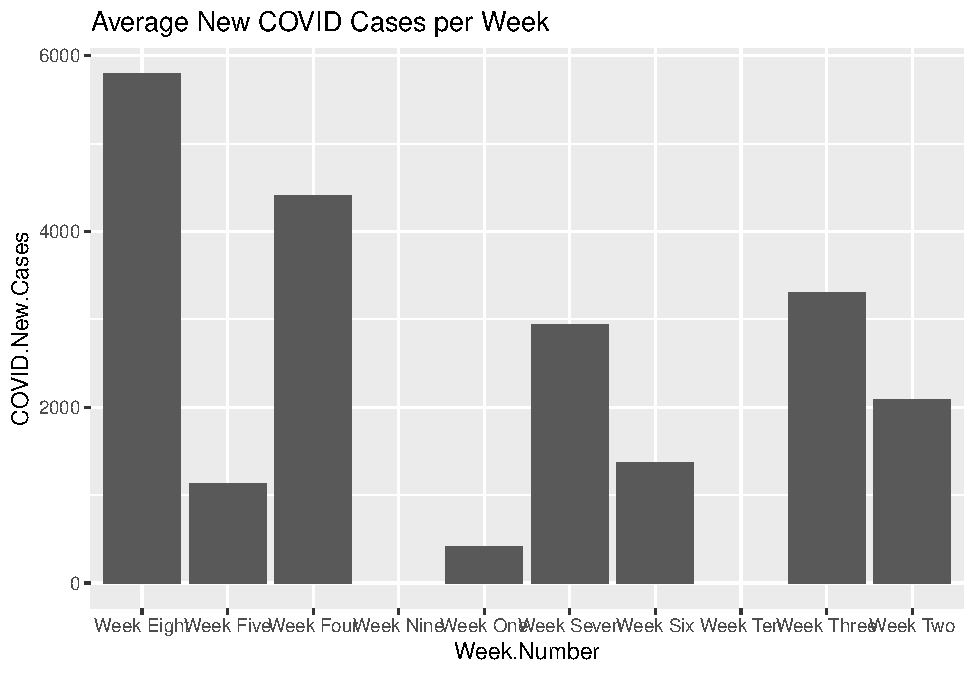
\includegraphics{project1_files/figure-latex/unnamed-chunk-4-4} \end{center}

A coorelation heatmap calculates an integer to represent the
relationship between variables. A number of ``1'' indicates sameness
between the two variables and any coorelation close to that is
considered to have a strong relationship. Some examples of this are seen
between the sum of COVID confirmed cases and the date. However, some
variables, such as the sum of COVID deaths and Sars new cases had a
correlation of ``0'', meaning there is no relationship between the two.
There were about equal distributions of strongly correlated variables as
well as variables that had weak correlations. Only a few would be
considered ``moderate'', as is seen between the sum of COVID confirmed
and COVID new cases.

The cases and deaths of Sars virus were plotted with the color of dot
indicating the week in which the deaths and cases occurred. The steepest
slope which indicated the highest death rate per sum of cases happened
around the onset of the virus and slowed toward its ending. There is a
positive relationship between the two variables indicated by the
positive slope of the line. As the sum of Sars deaths increased, the sum
of confirmed cases increased.

Box and whisker plots show summary statistics between variables. The box
itself indicates the IQR, representing the length between the lower and
upper quartile, the middle line indicates the median value, and the
whiskers show minimums and maximums. This third plot illustrated the sum
of COVID confirmed cases and sum of COVID deaths. As suspected, there
was a positive relationship between the two with a steady increase. As
can be seen by the spacing in the third plot, the highest increase in
deaths occurred between week seven and eight.

The final plot used stat=summary to find the mean of new COVID cases by
week number. Week one had the lowest average new cases, with week five
coming in at second lowest. The highest average new case count came from
week eight, with close to 6,000 new cases.

\begin{Shaded}
\begin{Highlighting}[]
\KeywordTok{library}\NormalTok{(cluster)}
\NormalTok{Clustered<-FULL_New}\OperatorTok\NormalTok{dplyr}\OperatorTok{::}\KeywordTok{select}\NormalTok{(}\OperatorTok{-}\NormalTok{Week.Number)}
\NormalTok{Clustered1<-Clustered}\OperatorTok\NormalTok{na.omit}\OperatorTok\NormalTok{scale}\OperatorTok\KeywordTok{as.data.frame}\NormalTok{()}
\NormalTok{sil_width<-}\KeywordTok{vector}\NormalTok{() }
\ControlFlowTok{for}\NormalTok{(i }\ControlFlowTok{in} \DecValTok{2}\OperatorTok{:}\DecValTok{10}\NormalTok{)\{}
\NormalTok{  kms <-}\StringTok{ }\KeywordTok{kmeans}\NormalTok{(Clustered1,}\DataTypeTok{centers=}\NormalTok{i) }
\NormalTok{  sil <-}\StringTok{ }\KeywordTok{silhouette}\NormalTok{(kms}\OperatorTok{$}\NormalTok{cluster,}\KeywordTok{dist}\NormalTok{(Clustered1)) }
\NormalTok{  sil_width[i]<-}\KeywordTok{mean}\NormalTok{(sil[,}\DecValTok{3}\NormalTok{])}
\NormalTok{\} }
\KeywordTok{ggplot}\NormalTok{()}\OperatorTok{+}\KeywordTok{geom_line}\NormalTok{(}\KeywordTok{aes}\NormalTok{(}\DataTypeTok{x=}\DecValTok{1}\OperatorTok{:}\DecValTok{10}\NormalTok{,}\DataTypeTok{y=}\NormalTok{sil_width))}\OperatorTok{+}\KeywordTok{scale_x_continuous}\NormalTok{(}\DataTypeTok{name=}\StringTok{"k"}\NormalTok{,}\DataTypeTok{breaks=}\DecValTok{1}\OperatorTok{:}\DecValTok{10}\NormalTok{)}
\end{Highlighting}
\end{Shaded}

\begin{center}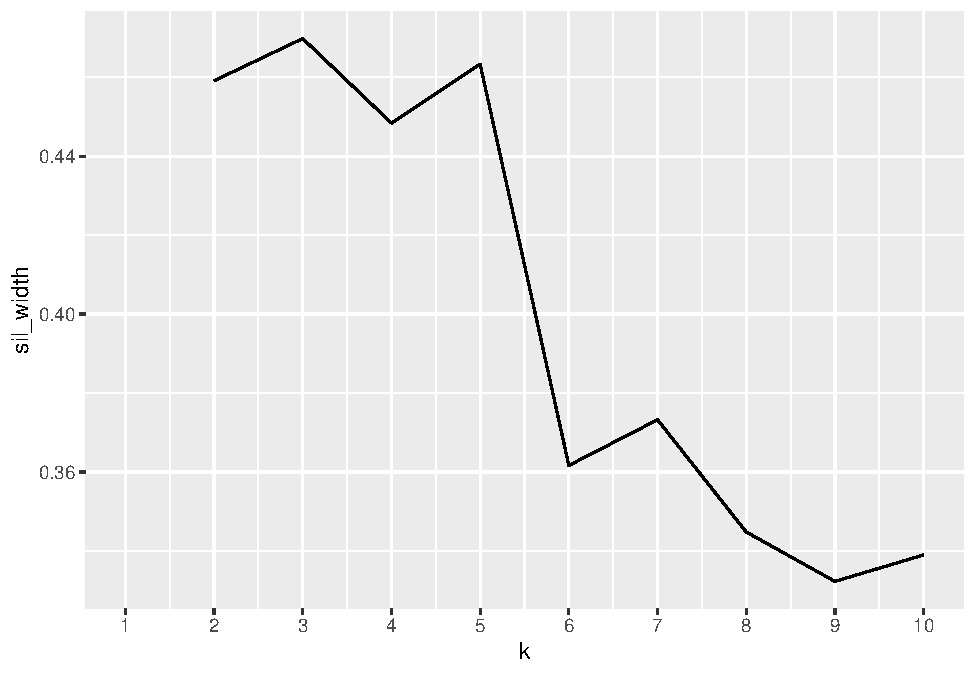
\includegraphics{project1_files/figure-latex/unnamed-chunk-5-1} \end{center}

\begin{Shaded}
\begin{Highlighting}[]
\NormalTok{pam1<-}\StringTok{ }\NormalTok{Clustered1 }\OperatorTok\StringTok{ }\KeywordTok{pam}\NormalTok{(}\DataTypeTok{k=}\DecValTok{2}\NormalTok{)}
\NormalTok{final<-Clustered1}\OperatorTok\KeywordTok{mutate}\NormalTok{(}\DataTypeTok{cluster=}\KeywordTok{as.factor}\NormalTok{(pam1}\OperatorTok{$}\NormalTok{clustering))}
\NormalTok{confmat<-final}\OperatorTok\KeywordTok{count}\NormalTok{(cluster)}\OperatorTok\KeywordTok{arrange}\NormalTok{(}\KeywordTok{desc}\NormalTok{(n))}\OperatorTok
\StringTok{  }\KeywordTok{pivot_wider}\NormalTok{(}\DataTypeTok{names_from=}\StringTok{"cluster"}\NormalTok{,}\DataTypeTok{values_from=}\StringTok{"n"}\NormalTok{,}\DataTypeTok{values_fill =} \KeywordTok{list}\NormalTok{(}\StringTok{'n'}\NormalTok{=}\DecValTok{0}\NormalTok{))}
\NormalTok{confmat}
\end{Highlighting}
\end{Shaded}

\begin{verbatim}
## # A tibble: 1 x 2
##     `1`   `2`
##   <int> <int>
## 1    27    25
\end{verbatim}

\begin{Shaded}
\begin{Highlighting}[]
\KeywordTok{ggplot}\NormalTok{(final, }\KeywordTok{aes}\NormalTok{(}\DataTypeTok{x=}\NormalTok{Sum.of.COVID.Deaths,}\DataTypeTok{y=}\NormalTok{Sum.of.Sars.Deaths, }\DataTypeTok{color=}\NormalTok{cluster))}\OperatorTok{+}\KeywordTok{geom_point}\NormalTok{()}
\end{Highlighting}
\end{Shaded}

\begin{center}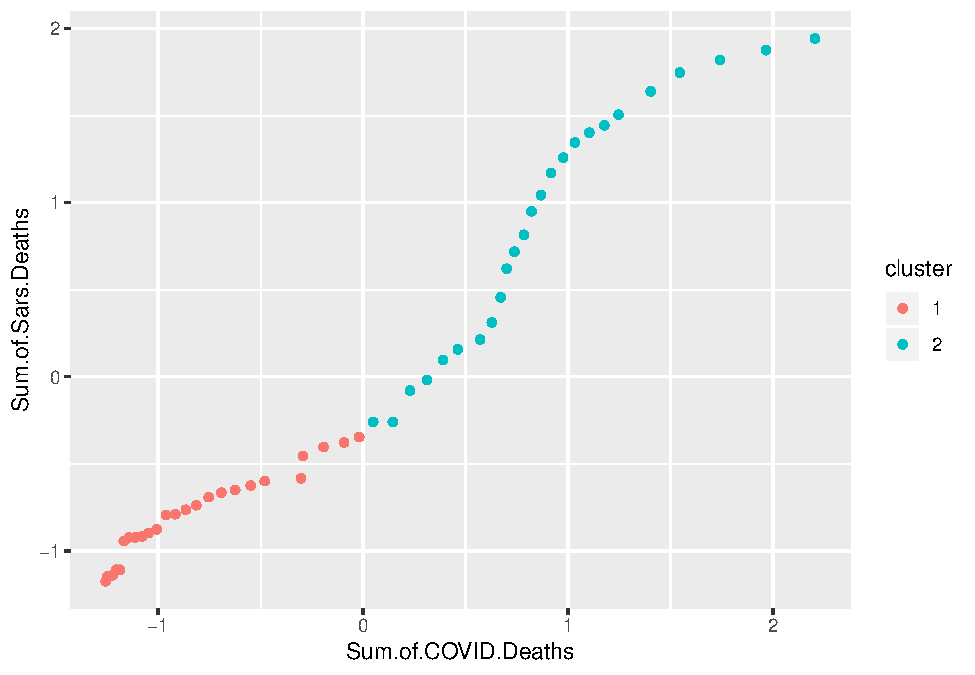
\includegraphics{project1_files/figure-latex/unnamed-chunk-5-2} \end{center}

\begin{Shaded}
\begin{Highlighting}[]
\KeywordTok{plot}\NormalTok{(pam1, }\DataTypeTok{which=}\DecValTok{2}\NormalTok{)}
\end{Highlighting}
\end{Shaded}

\begin{center}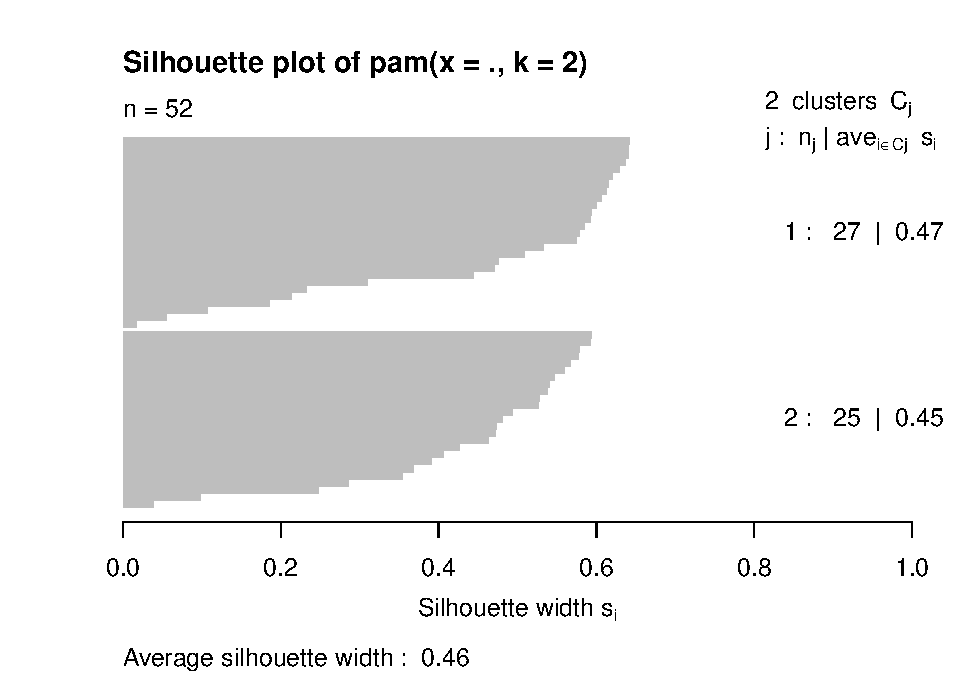
\includegraphics{project1_files/figure-latex/unnamed-chunk-5-3} \end{center}

According to the ggplot, the highest average silhouette width came from
five clusters (.463), but the second highest was very close and
suggested two (.459). Given it is better to choose fewer clusters to
achieve parsimony, I decided to have two. The quantity of clusters
recommended was based on all numeric variables in the dataset, but only
the sums of COVID deaths and Sars deaths were visualized. As seen on the
ggplot, there were no real ``clusters'' or clear separation, but more
evenly spaced out points throughout the graph. Given the silhouette
width used to derive the clusters was not very high, the cluster
solution achieved did not elicit much information.

\end{document}
